\documentclass[a4paper]{article}

\usepackage[margin=1in]{geometry} 
\usepackage{amsmath,amsthm,amssymb}
\usepackage{float}
\usepackage{graphicx}
\usepackage{xcolor}
\usepackage[UKenglish]{isodate}
\origdate
\cleanlookdateon
\usepackage[utf8]{inputenc}
\usepackage[hidelinks]{hyperref}
\usepackage{tikz-cd}
\usepackage{enumitem}
\usepackage{mathtools}
\usepackage{pgfplots}
\usepackage{float}
\usepackage{tikz, venndiagram}
\usepackage{tkz-euclide}
\usepackage{tabu}
\usepackage{framed}
\usepackage{steinmetz}
\renewcommand{\baselinestretch}{1.5} 
\usepackage[varg]{txfonts}
\usepackage{microtype}
\usepackage{mathrsfs} 
\usepackage{makecell}
\usepackage{tocloft}
\addtolength{\cftsubsecnumwidth}{10pt}

\pgfplotsset{compat=1.16}
\begin{document}
\title{Finals Revision Guide\\[0.1cm]
    \large 30.102 Electromagnetics \& Applications, Term 5 2020}
\author{Wei Min Cher}
\date{21 Apr 2020}

\maketitle

\tableofcontents

\newpage
\section{W6: Vector Algebra}

\subsection{Orthogonal Coordinate Systems}

\subsubsection{Cartesian Coordinates}
\begin{itemize}
    \item Coordinate variables: $x$, $y$, $z$
\end{itemize}

\subsubsection{Cylindrical Coordinates}
\begin{itemize}
    \item Coordinate variables:
    \begin{itemize}[label=$\circ$]
        \item $r$: radial distance in $x$-$y$ plane, \quad $0\leq r \leq \infty$
        \item $\phi$: azimuth angle from positive $x$-axis, \quad $0\leq\phi\leq 2\pi$
        \item $z$: defined in Cartesian coordinate system, \quad $-\infty\leq z\leq\infty$
    \end{itemize}
\end{itemize}

\subsubsection{Spherical Coordinates}
\begin{itemize}
    \item Coordinate variables:
    \begin{itemize}[label=$\circ$]
        \item $R$: range coordinate, \quad $0\leq R\leq \infty$
        \item $\theta$: zenith angle from positive $z$-axis, \quad $0\leq\theta\leq\pi$
        \item $\phi$: azimuth angle from positive $x$-axis, \quad $0\leq\phi\leq 2\pi$
    \end{itemize}
\end{itemize}

\subsubsection{Summary for Vectors in Coordinate Systems}
\begin{table}[H]
\centering
\begin{tabular}{l|c|c|c|}
\cline{2-4}
 & \textbf{Cartesian} & \textbf{Cylindrical} & \textbf{Spherical} \\ \hline
\multicolumn{1}{|l|}{Coordinate variables} & $x,\ y,\ z$ & $r,\ \phi,\ z$ & $R,\ \theta,\ \phi$ \\ \hline
\multicolumn{1}{|l|}{Position vector, $\overrightarrow{OP_1}$} & \begin{tabular}[c]{@{}c@{}}$\hat{x}x_1+\hat{y}y_1+\hat{z}z_1$\\ for P($x_1,\ y_1,\ z_1$)\end{tabular} & \begin{tabular}[c]{@{}c@{}}$\hat{r}r_1+\hat{z}z_1$\\ for P($r_1,\ \phi_1,\ z_1$)\end{tabular} & \begin{tabular}[c]{@{}c@{}}$\hat{R}R_1$\\ for P($R_1,\ \theta_1,\ \phi_1$)\end{tabular} \\ \hline
\multicolumn{1}{|l|}{Unit vector operations} & \begin{tabular}[c]{@{}c@{}}$\hat{x}\cdot\hat{x} = \hat{y}\cdot\hat{y} = \hat{z}\cdot\hat{z} = 1$\\ $\hat{x}\cdot\hat{y} = \hat{y}\cdot\hat{z} = \hat{z}\cdot\hat{x} = 0$\\ $\hat{x}\times\hat{y} = \hat{z}$\\ $\hat{y}\times\hat{z} = \hat{x}$\\ $\hat{z}\times\hat{x} = \hat{y}$\end{tabular} & \begin{tabular}[c]{@{}c@{}}$\hat{r}\cdot\hat{r} = \hat{\phi}\cdot\hat{\phi} = \hat{z}\cdot\hat{z} = 1$\\ $\hat{r}\cdot\hat{\phi} = \hat{\phi}\cdot\hat{z} = \hat{z}\cdot\hat{r} = 0$\\ $\hat{r}\times\hat{\phi} = \hat{z}$\\ $\hat{\phi}\times\hat{z} = \hat{r}$\\ $\hat{z}\times\hat{r} = \hat{\phi}$\end{tabular} & \begin{tabular}[c]{@{}c@{}}$\hat{R}\cdot\hat{R} = \hat{\theta}\cdot\hat{\theta} = \hat{\phi}\cdot\hat{\phi} = 1$\\ $\hat{R}\cdot\hat{\theta} = \hat{\theta}\cdot\hat{\phi} = \hat{\phi}\cdot\hat{R} = 0$\\ $\hat{R}\times\hat{\theta} = \hat{\phi}$\\ $\hat{\theta}\times\hat{\phi} = \hat{R}$\\ $\hat{\phi}\times\hat{R} = \hat{\theta}$\end{tabular} \\ \hline
\multicolumn{1}{|l|}{Dot product, $\overrightarrow{A}\cdot\overrightarrow{B}$} & $A_x B_x+A_y B_y+A_z B_z$ & $A_r B_r+A_\phi B_\phi+A_z B_z$ & $A_RB_R+A_\theta B_\theta+A_\phi B_\phi$ \\ \hline
\multicolumn{1}{|l|}{Cross product, $\overrightarrow{A}\times\overrightarrow{B}$} & $\begin{vmatrix}\hat{x}&\hat{y}&\hat{z}\\A_x&A_y&A_z\\B_x&B_y&B_z\end{vmatrix}$ & $\begin{vmatrix}\hat{r}&\hat{\phi}&\hat{z}\\A_r&A_\phi&A_z\\B_r&B_\phi&B_z\end{vmatrix}$ & $\begin{vmatrix}\hat{R}&\hat{\theta}&\hat{\phi}\\A_R&A_\theta&A_\phi\\B_R&B_\theta&B_\phi\end{vmatrix}$ \\ \hline
\multicolumn{1}{|l|}{Differential length, $d\vec{l}$} & $\hat{x}\ dx+\hat{y}\ dy+\hat{z}\ dz$ & $\hat{r}\ dr+\hat{\phi}r\ d\phi+\hat{z}\ dz$ & $\hat{R}\ dR+\hat{\theta}R\ d\theta+\hat{\phi}R\sin\theta\ d\phi$ \\ \hline
\multicolumn{1}{|l|}{Differential areas} & \begin{tabular}[c]{@{}c@{}}$d_{\overrightarrow{s_x}} = \hat{x}\ dy\ dz$\\ $d_{\overrightarrow{s_y}} = \hat{y}\ dx\ dz$\\ $d_{\overrightarrow{s_z}} = \hat{z}\ dx\ dy$\end{tabular} & \begin{tabular}[c]{@{}c@{}}$d_{\overrightarrow{s_r}} = \hat{r}r\ d\phi\ dz$\\ $d_{\overrightarrow{s_\phi}} = \hat{r}r\ d\phi\ dz$\\ $d_{\overrightarrow{s_z}} = \hat{z}r\ dr\ d\phi$\end{tabular} & \begin{tabular}[c]{@{}c@{}}$d_{\overrightarrow{s_R}} = \hat{R}R^2\sin\theta\ d\theta\ d\phi$\\ $d_{\overrightarrow{s_\theta}} = \hat{\theta}R\sin\theta\ dR\ d\phi$\\ $d_{\overrightarrow{s_\phi}} = \hat{\phi}R\ dR\ d\theta$\end{tabular} \\ \hline
\multicolumn{1}{|l|}{Differential volume, $d\vec{V}$} & $dx\ dy\ dz$ & $r\ dr\ d\phi\ dz$ & $R^2\sin\theta\ dR\ d\theta\ d\phi$ \\ \hline
\end{tabular}
\end{table}

\subsection{Transformation between Coordinate Systems}
\begin{table}[H]
\setcellgapes{1pt}
\centering\makegapedcells
\begin{tabular}{|l|l|l|}
\hline
\multicolumn{1}{|c|}{\textbf{Transformation}} & \multicolumn{1}{c|}{\textbf{Coordinate Variables}} & \multicolumn{1}{c|}{\textbf{Unit Vectors}} \\ \hline
Cartesian $\rightarrow$ cylindrical & \begin{tabular}[c]{@{}l@{}}$r = \sqrt{x^2+y^2}$\\ $\phi = \tan^{-1}\left(\displaystyle\frac{y}{x}\right)$\end{tabular} & \begin{tabular}[c]{@{}l@{}}$\hat{r} = \hat{x}\cos\phi+\hat{y}\sin\phi$\\ $\hat{\phi} = -\hat{x}\sin\phi+\hat{y}\cos\phi$\end{tabular} \\ \hline
Cylindrical $\rightarrow$ Cartesian & \begin{tabular}[c]{@{}l@{}}$x = r\cos\phi$\\ $y = r\sin\phi$\end{tabular} & \begin{tabular}[c]{@{}l@{}}$\hat{x} = \hat{r}\cos\phi-\hat{\phi}\sin\phi$\\ $\hat{y} = \hat{r}\sin\phi+\hat{\phi}\cos\phi$\end{tabular} \\ \hline
Cartesian $\rightarrow$ spherical & \begin{tabular}[c]{@{}l@{}}$R = \sqrt{x^2+y^2+z^2}$\\ $\theta = \tan^{-1}\left(\displaystyle\frac{\sqrt{x^2+y^2}}{z}\right)$\\ $\phi = \tan^{-1}\left(\displaystyle\frac{y}{x}\right)$\end{tabular} & \begin{tabular}[c]{@{}l@{}}$\hat{R} = \hat{x}\sin\theta\cos\phi+\hat{y}\sin\theta\sin\phi+\hat{z}\cos\theta$\\ $\hat{\theta} = \hat{x}\cos\theta\cos\phi+\hat{y}\cos\theta\sin\phi-\hat{z}\sin\theta$\\ $\hat{\phi} = -\hat{x}\sin\phi+\hat{y}\cos\phi$\end{tabular} \\ \hline
Spherical $\rightarrow$ Cartesian & \begin{tabular}[c]{@{}l@{}}$x = R\sin\theta\cos\phi$\\ $y = R\sin\theta\sin\phi$\\ $z = R\cos\theta$\end{tabular} & \begin{tabular}[c]{@{}l@{}}$\hat{x} = \hat{R}\sin\theta\cos\phi+\hat{\theta}\cos\theta\cos\phi-\hat{\phi}\sin\phi$\\ $\hat{y} = \hat{R}\sin\theta\sin\phi+\hat{\theta}\cos\theta\sin\phi+\hat{\phi}\sin\phi$\\ $\hat{z} = \hat{R}\cos\theta-\hat{\theta}\sin\theta$\end{tabular} \\ \hline
Cylindrical $\rightarrow$ spherical & \begin{tabular}[c]{@{}l@{}}$R = \sqrt{r^2+z^2}$\\ $\theta = \tan^{-1}\left(\displaystyle\frac{r}{z}\right)$\end{tabular} & \begin{tabular}[c]{@{}l@{}}$\hat{R} = \hat{r}\sin\theta+\hat{z}\cos\theta$\\ $\hat{\theta} = \hat{r}\cos\theta-\hat{z}\sin\theta$\end{tabular} \\ \hline
Spherical $\rightarrow$ cylindrical & \begin{tabular}[c]{@{}l@{}}$r = R\sin\theta$\\ $z = R\cos\theta$\end{tabular} & \begin{tabular}[c]{@{}l@{}}$\hat{r} = \hat{R}\sin\theta+\hat{\theta}\cos\theta$\\ $\hat{z} = \hat{R}\cos\theta-\hat{\theta}\sin\theta$\end{tabular} \\ \hline
\end{tabular}
\end{table}

\subsection{Distance between Two Points}
\begin{itemize}
    \item Cartesian coordinates:
    $$d = \sqrt{(x_2-x_1)^2+(y_2-y_1)^2+(z_2-z_1)^2}$$
    \item Cylindrical coordinates:
    $$d = \sqrt{r_2^2+r_1^2-2r_1r_2\cos(\phi_2-\phi_1)+(z_2-z_1)^2}$$
    \item Spherical coordinates:
    $$d = \sqrt{R_2^2+R_1^2-2R_1R_2\left[\cos\theta_2\cos\theta_1+\sin\theta_1\sin\theta_2\cos(\phi_2-\phi_1)\right]}$$
\end{itemize}

\subsection{Gradient of Scalar Field}
\begin{itemize}
    \item Gradient of $T$, $\nabla T$
    $$\nabla T = \hat{u}_1\frac{\partial T}{h_1\partial u_1}+\hat{u}_2\frac{\partial T}{h_2\partial u_2}+\hat{u}_3\frac{\partial T}{h_3\partial u_3}$$
    \item Directional directive of $T$ along $\hat{a}_l$, $\displaystyle\frac{dT}{dl}$
    $$\frac{dT}{dl} = \nabla T\cdot \hat{a}_l$$
\end{itemize}

\subsection{Divergence of Vector Field}
\begin{itemize}
    \item Divergence of $\overrightarrow{E}$, $\nabla\cdot\overrightarrow{E}$
    $$\nabla\cdot\overrightarrow{E} = \frac{1}{h_1h_2h_3}\left[\frac{\partial}{\partial u_1}(h_2h_3E_1)+\frac{\partial}{\partial u_2}(h_3h_1E_2)+\frac{\partial}{\partial u_3}(h_1h_2E_3)\right]$$
    \item Divergence Theorem
    $$\int\limits_\mathcal{V} \nabla\cdot\overrightarrow{E}\ d\mathcal{V} = \oint\limits_S \overrightarrow{E}\cdot d\vec{s}$$
\end{itemize}

\subsection{Curl of Vector Field}
\begin{itemize}
    \item Curl of $\overrightarrow{B}$, $\nabla\times\overrightarrow{B}$
    $$\nabla\times\overrightarrow{B} = \frac{1}{h_1h_2h_3}\left|
    \begin{array}{ccc}
         h_1\hat{u}_1 & h_2\hat{u}_2 & h_3\hat{u}_3\\
         \frac{\partial}{\partial u_1}& \frac{\partial}{\partial u_2} & \frac{\partial}{\partial u_3}\\
         h_1H_1 & h_2H_2 & h_3H_3
    \end{array}\right|$$
    \item Stokes' Theorem
    $$\int\limits_{S}(\nabla\times\overrightarrow{B})\cdot d\vec{s} = \oint\limits_{C} \overrightarrow{B}\cdot d\vec{l}$$
\end{itemize}

\subsection{Laplacian Operator}
\begin{itemize}
    \item Laplacian of scalar field, $V$
    $$\nabla^2 V = \nabla\cdot(\nabla V) = \frac{1}{h_1h_2h_3}\left[\frac{\partial}{\partial u_1}h_2h_3\frac{\partial V}{h_1\partial u_1}+\frac{\partial}{\partial u_2}h_3h_1\frac{\partial V}{h_2\partial u_2}+\frac{\partial}{\partial u_3}h_1h_2\frac{\partial V}{h_3\partial u_3}\right]$$
    \item Laplacian of vector field, $\overrightarrow{E}$
    $$\nabla^2 \overrightarrow{E} = \left(\frac{\partial^2}{\partial x^2}+\frac{\partial^2}{\partial y^2}+\frac{\partial^2}{\partial z^2}\right)\overrightarrow{E}$$
    \item Relation between dot and cross products
    $$\nabla^2\overrightarrow{E} = \nabla(\nabla\cdot\overrightarrow{E})-\nabla\times(\nabla\times\overrightarrow{E})$$
\end{itemize}

\subsection{Summary for Advanced Vector Operations}
\begin{table}[H]
\centering
\begin{tabular}{|c|c|c|c|}
\hline
\begin{tabular}[c]{@{}c@{}}Orthogonal \\ Coordinate System\end{tabular} & Cartesian & Cylindrical & Spherical \\ \hline
\begin{tabular}[c]{@{}c@{}}Base Vectors\\ ($\hat{u}_1,\ \hat{u}_2,\ \hat{u}_3$)\end{tabular} & $\hat{x},\ \hat{y},\ \hat{z}$ & $\hat{r},\ \hat{\phi},\ \hat{z}$ & $\hat{R},\ \hat{\theta},\ \hat{\phi}$ \\ \hline
\begin{tabular}[c]{@{}c@{}}Metric Coefficients\\ ($h_1,\ h_2,\ h_3$)\end{tabular} & 1, 1, 1 & $1,\ r,\ 1$ & $1,\ R,\ R\sin\theta$ \\ \hline
\begin{tabular}[c]{@{}c@{}}Differential Volume\\ ($h_1h_2h_3\ du_1\ du_2\ du_3$)\end{tabular} & $dx\ dy\ dz$ & $r\ dr\ d\phi\ dz$ & $R^2\sin\theta\ dR\ d\theta\ d\phi$ \\ \hline
\end{tabular}
\end{table}

\newpage
\section{W8: Physics II Review} 
\subsection{Epsilon \& Mu}
\begin{itemize}
    \item Electric flux density, $\overrightarrow{D} = \epsilon\overrightarrow{E}$, measured in C/$\text{m}^2$
    \item Magnetic flux density, $\overrightarrow{B} = \mu\overrightarrow{H}$, measured in T
\end{itemize}

\subsection{Static \& Dynamic Fields}
\begin{itemize}
    \item Standard conditions:
    \begin{itemize}[label=$\circ$]
        \item Electric and magnetic fields are independent
    \end{itemize}
    \item Dynamic conditions:
    \begin{itemize}[label=$\circ$]
        \item Electric and magnetic fields are coupled
    \end{itemize}
\end{itemize}

\subsection{Faraday's Law}
$$\oint\limits_C \overrightarrow{E}\cdot d\vec{l} = -\frac{d}{dt}\int\limits_S \overrightarrow{B}\cdot d\vec{s}$$
\begin{itemize}
    \item 3 scenarios:
    \begin{enumerate}
        \item Time-varying magnetic field linking stationary loop
        $$\text{Induced transformer emf, }V_{emf}^{tr} = -N\int\limits_{S}\frac{d\vec{B}}{dt}\cdot d\vec{s}\ \text{ (V)}$$
        \item Moving loop with time-varying surface area relative to the normal of $\overrightarrow{B}$
        $$\text{Induced motional emf, }V_{emf}^{m} = \oint\limits_{C}\ (\overrightarrow{u}\times\overrightarrow{B})\cdot d\vec{l}\ \text{ (V)}$$
        \begin{itemize}[label=$\circ$]
            \item where $\overrightarrow{u}$ is the velocity of the moving particle
        \end{itemize}
        \item Moving loop in a time-varying field $\overrightarrow{B}$
        $$\text{Total emf, }V_{emf} = V_{emf}^{tr}+V_{emf}^{m}$$
    \end{enumerate}
    \item Using Stoke's Theorem, it can be expressed in differential form as \boxed{\nabla\times\overrightarrow{E} = -\frac{\partial\overrightarrow{B}}{\partial t}}\ .
\end{itemize}

\subsection{Maxwell-Ampere's Law}
\begin{align*}
    \oint\limits_{C}\ \overrightarrow{B}\cdot d\vec{l} &= \mu_0\iint\limits_{S}\overrightarrow{J}\cdot\hat{n}\ d\vec{s}+\epsilon_0\mu_0\frac{d}{dt}\iint\limits_{S}\overrightarrow{E}\cdot\hat{n}\ d\vec{s}\\
    &= \mu_0(I_c+I_d)
\end{align*}
\begin{itemize}
    \item Enclosed current, $I_c = \iint\limits_{S}\overrightarrow{J}\cdot\hat{n}\ d\vec{s}$
    \item Displacement current, $I_d = \epsilon_0\displaystyle\frac{d}{dt}\iint\limits_{S}\overrightarrow{E}\cdot\hat{n}\ d\vec{s}$
    \item Using Stoke's Theorem, it can be expressed in differential form as \boxed{\nabla\times\overrightarrow{H} = \overrightarrow{J}+\frac{d\vec{D}}{dt}}\ .
\end{itemize}

\subsection{Gauss' Law}
$$\oint\limits_{S}\ \overrightarrow{D}\cdot d\vec{s} = \int\limits_{V}\rho d\vec{V}$$
\begin{itemize}
    \item Using Divergence Theorem, it can be expressed in differential form as \boxed{\nabla\cdot\overrightarrow{D} = \rho}\ .
\end{itemize}

\subsection{Gauss' Law for Magnetism}
$$\oint\limits_{S}\ \overrightarrow{B}\cdot d\vec{s} = 0$$
\begin{itemize}
    \item Using Divergence Theorem, it can be expressed in differential form as \boxed{\nabla\cdot\overrightarrow{B} = 0}\ .
\end{itemize}

\newpage
\section{W10 - W11: Plane Waves}

\subsection{Complex Permittivity}
\begin{itemize}
    \item Complex permittivity, $\epsilon_c = \epsilon-j\displaystyle\frac{\sigma}{\omega}$
    \begin{itemize}[label=$\circ$]
        \item Real part, $\epsilon' = \epsilon$
        \item Complex part, $\epsilon'' = \displaystyle\frac{\sigma}{\omega}$
        \item If lossless, $\epsilon'' = 0,\ \epsilon_c = \epsilon$.
    \end{itemize}
    \item Loss tangent, $\tan\delta = \displaystyle\frac{\epsilon''}{\epsilon'} = \displaystyle\frac{\sigma}{\omega\epsilon}$
\end{itemize}

\subsection{Wave Equations}
\begin{center}
    \boxed{\begin{array}{cc}
         \nabla^2\widetilde{E}-\gamma^2\widetilde{E} = 0 & \text{ for }\widetilde{E}  \\
         \nabla^2\widetilde{H}-\gamma^2\widetilde{H} = 0 & \text{ for }\widetilde{H} 
    \end{array}}
\end{center}

\subsection{Wave Equations in Lossless Media}
\begin{itemize}
    \item Wave number, $k= \omega\sqrt{\mu\epsilon}$
    \begin{itemize}[label=$\circ$]
        \item In lossless medium, $\gamma^2 = -k^2$.
        \begin{center}
            \boxed{\begin{array}{c}
                 \nabla^2\widetilde{E}+k^2\widetilde{E} = 0 \\
                 \nabla^2\widetilde{B}+k^2\widetilde{B} = 0
            \end{array}}
        \end{center}
        \item Known as $\beta$ in lossy medium.
    \end{itemize}
\end{itemize}

\subsection{Intrinsic Impedance of Lossless Medium}
\begin{itemize}
    \item Intrinsic impedance of lossless medium, $\eta$
    \begin{center}
        \boxed{\eta = \frac{E_{x0}^+}{H_{y0}^+} = \frac{\omega\mu}{k} = \frac{\omega\mu}{\omega\sqrt{\mu\epsilon}} = \sqrt{\frac{\mu}{\epsilon}}\ (\Omega)}
    \end{center}
\end{itemize}

\subsection{Phase Velocity}
$$\text{Phase velocity, }u_p = \frac{\omega}{k} = \frac{\omega}{\omega\sqrt{\mu\epsilon}} = \frac{1}{\sqrt{\mu\epsilon}}\text{ (m/s)}$$
\begin{itemize}
    \item In vacuum: $\epsilon = \epsilon_0,\ \mu = \mu_0$
    $$\Rightarrow u_p = \frac{1}{\sqrt{\epsilon_0\mu_0}} = 3\times10^8\text{ m/s}$$
\end{itemize}

\subsection{Intrinsic Impedance of Free Space}
$$\text{Intrinsic impedance of free space, }\eta_0 = \sqrt{\frac{\mu_0}{\epsilon_0}} = 377\ \Omega \approx 120\pi\ \Omega$$

\subsection{Transverse Electromagnetic Waves (TEM)}
\begin{itemize}
    \item Generally, $\widetilde{E}$ and $\widetilde{H}$ can be described in terms of $\widetilde{k}$:
    \begin{center}
    \boxed{\begin{array}{c}
         \widetilde{H} = \displaystyle\frac{1}{\eta}\hat{k}\times\widetilde{E} \\
          \widetilde{E} = -\eta\hat{k}\times\widetilde{H}
    \end{array}}
    \end{center}
    \item If $\widetilde{E}$ has a component in positive $x$-direction and is travelling in the z-direction, then
     \begin{center}
    \boxed{\begin{array}{cc}
         \widetilde{E}(z) = \hat{x}\widetilde{E}_x^+(z), & \widetilde{H}(z) = \hat{y}\displaystyle\frac{\widetilde{E}_x^+(z)}{\eta}\\
         \widetilde{H}_x^+ = -\displaystyle\frac{\widetilde{E}_y^+(z)}{\eta}, & \widetilde{H}_y^+ = \displaystyle\frac{\widetilde{E}_x^+(z)}{\eta}
    \end{array}}\ .
    \end{center}
\end{itemize}

\subsection{Instantaneous Electric and Magnetic Fields}
\begin{itemize}
    \item $E_{x0}^+$ is a complex quantity with magnitude $|E_{x0}^+|$ and phase angle $\phi^+$.
    $$E_{x0}^+ = |E_{x0}^+|e^{j\phi^+}$$
    \item Instantaneous electric field $\overrightarrow{E}(z, t)$
    $$\overrightarrow{E}(z, t) = \operatorname{Re}\left[\widetilde{E}(z)e^{j\omega t}\right] = \hat{x}|E_{x0}^+|\cos(\omega t-kz+\phi^+)\ \text{ (V/m)}$$
    \item Instantaneous magnetic field $\overrightarrow{H}(z, t)$
    $$\overrightarrow{E}(z, t) = \operatorname{Re}\left[\widetilde{H}(z)e^{j\omega t}\right] = \hat{x}\frac{|E_{x0}^+|}{\eta}\cos(\omega t-kz+\phi^+)\ \text{ (A/m)}$$
\end{itemize}

\subsection{Polarization}
\begin{itemize}
    \item Polarization: describes locus traced by tip of $\overrightarrow{E}$ at given point in space as function of time
    \item Types: linear, circular, elliptical
    \bigskip
    \item For $\widetilde{E}$ propagating in $z$-direction, we can express it in terms of $\widetilde{E}_x$ and $\widetilde{E}_y$.
    $$\widetilde{E}(z) = \hat{x}\widetilde{E}_x(z)+\hat{y}\widetilde{E}_y(z) = (\hat{x}a_x+\hat{y}a_ye^{j\delta})e^{-jkz}$$
    \begin{itemize}[label=$\circ$]
        \item where $\widetilde{E}_x(z) = E_{x0}e^{-jkz} = a_xe^{-jkz}$,
        \item and $\widetilde{E}_y(z) = E_{y0}e^{-jkz} = a_xe^{j\delta}e^{-jkz}$.
    \end{itemize}
    \item Instantaneous electric field $\overrightarrow{E}(z, t)$
    \begin{align*}
        \overrightarrow{E}(z, t) &= \operatorname{Re}\left[\widetilde{E}(z)e^{j\omega t}\right]\\
        &= \hat{x}a_x\cos(\omega t-kz)+\hat{y}a_y\cos(\omega t-kz+\delta)
    \end{align*}
    \item Magnitude of electric field $|\overrightarrow{E}(z, t)|$
    \begin{align*}
        |\overrightarrow{E}(z, t)| &= \sqrt{E_x^2(z, t)+E_y^2(z, t)}\\
        &= \sqrt{a_x^2\cos^2(\omega t-kz)+a_y^2\cos^2(\omega-kz+\delta)}
    \end{align*}
    \item Inclination angle $\psi(z, t)$
    $$\psi(z, t) = \tan^{-1}\left(\frac{E_y(z, t)}{E_x(z, t)}\right)$$
\end{itemize}

\subsubsection{Linear Polarization}
\begin{itemize}
    \item When $\delta = 0$ (in phase):
    $$\begin{array}{c}
         \overrightarrow{E}(z, t) = (\hat{x}a_x+\hat{y}a_y)\cos(\omega t-kz)\\
         |\overrightarrow{E}(z, t) = \sqrt{a_x^2+a_y^2}\cos(\omega t-kz)\\
         \psi(z, t) = \tan^{-1}\left(\displaystyle\frac{a_y}{a_x}\right)
    \end{array}$$
    \item When $\delta = \pi$ (out of phase):
    $$\begin{array}{cc}
         \overrightarrow{E}(z, t) = (\hat{x}a_x-\hat{y}a_y)\cos(\omega t-kz)\\
         |\overrightarrow{E}(z, t) = \sqrt{a_x^2+a_y^2}\cos(\omega t-kz)\\
         \psi(z, t) = \tan^{-1}\left(\displaystyle\frac{-a_y}{a_x}\right)
    \end{array}$$
    \item $|\overrightarrow{E}(z, t)|$ is changing over time
    \item $\psi$ is independent of $z$ and $t$ $\Rightarrow$ inclination angle is fixed 
    \item When $a_y = 0,\ \psi = 0^\circ$ or $180^\circ$, the wave is x-polarized.
    \item When $a_x = 0,\ \psi = \pm 90^\circ$, the wave is y-polarized.
\end{itemize}

\subsubsection{Circular Polarization}
\begin{itemize}
    \item When $\delta = \displaystyle\frac{\pi}{2}$ (left-hand circular polarization):
    $$\begin{array}{c}
         \overrightarrow{E}(z, t) = \hat{x}\ a\cos(\omega t-kz)-\hat{y}\ a \sin(\omega t-kz)\\
         |\overrightarrow{E}(z, t)| = a\\
         \psi(z, t) = -(\omega t-kz)
    \end{array}$$
    \item When $\delta = \displaystyle-\frac{\pi}{2}$ (right-hand circular polarization):
    $$\begin{array}{c}
         \overrightarrow{E}(z, t) = \hat{x}\ a\cos(\omega t-kz)+\hat{y}\ a \sin(\omega t-kz)\\
         |\overrightarrow{E}(z, t)| = a\\
         \psi(z, t) = \omega t-kz
    \end{array}$$
    \item $\overrightarrow{E}(z, t)$ is independent of $z$ and $t$ $\Rightarrow$ magnitude is fixed
    \item $\psi$ is changing over time
\end{itemize}

\newpage
\subsection{Plane Waves in Lossy Media}
\begin{itemize}
    \item General equations for $\alpha$ and $\beta$:
    \begin{center}
        \boxed{$$\begin{array}{c}
             \alpha = \omega\left\{\displaystyle\frac{\mu\epsilon'}{2}\left[\sqrt{1+\left(\displaystyle\frac{\epsilon''}{\epsilon'}\right)^2-1}\right]\right\}^{1/2}\text{ (Np/m)} \\
             \beta = \omega\left\{\displaystyle\frac{\mu\epsilon'}{2}\left[\sqrt{1+\left(\displaystyle\frac{\epsilon''}{\epsilon'}\right)^2+1}\right]\right\}^{1/2}\text{ (rad/m)} 
        \end{array}$$}
    \end{center}
    \item Intrinsic impedance of lossy medium, $\eta_c$
    $$\eta_c = \sqrt{\frac{\mu}{\epsilon_c}} = \sqrt{\frac{\mu}{\epsilon}}\left(1-j\frac{\epsilon''}{\epsilon'}\right)^{-1/2}\ (\Omega)$$
    \item Approximations can be made:
    \begin{itemize}[label=$\circ$]
        \item If $\displaystyle\frac{\epsilon''}{\epsilon'} \ll 1$, material is a low-loss dielectric.
        \item If $\displaystyle\frac{\epsilon''}{\epsilon'} \gg 1$, material is a good conductor.
    \end{itemize}
\end{itemize}

\subsubsection{Low-Loss Dielectric}
\begin{center}
        \boxed{$$\begin{array}{c}
             \alpha \approx\displaystyle\frac{\omega\epsilon''}{2}\sqrt{\displaystyle\frac{\mu}{\epsilon'}} = \displaystyle\frac{\sigma}{2}\sqrt{\displaystyle\frac{\mu}{\epsilon}}\ \text{ (Np/m)} \\[0.25cm]
             \beta \approx \omega\sqrt{\mu\epsilon'} = \omega\sqrt{\mu\epsilon}\ \text{ (rad/m)}\\[0.25cm]
             \eta_c \approx \sqrt{\displaystyle\frac{\mu}{\epsilon}}\ (\Omega)
        \end{array}$$}
\end{center}

\subsubsection{Good Conductor}
\begin{center}
        \boxed{$$\begin{array}{c}
             \alpha \approx\omega\sqrt{\displaystyle\frac{\mu\epsilon''}{2}} = \omega\sqrt{\displaystyle\frac{\mu\sigma}{2\omega}} = \sqrt{\pi f\mu\sigma}\ \text{ (Np/m)} \\[0.25cm]
             \beta\approx\alpha=\sqrt{\pi f\mu\sigma}\ \text{ (rad/m)}\\[0.25cm]
             \eta_c \approx \sqrt{j\displaystyle\frac{\mu}{\epsilon''}} = (1+j)\sqrt{\displaystyle\frac{\pi f\mu}{\sigma}} = (1+j)\displaystyle\frac{\alpha}{\sigma}\ (\Omega)\\[0.25cm]
             u_p = \sqrt{\displaystyle\frac{4\pi f}{\mu\sigma}}\ \text{ (m/s)}
        \end{array}$$}
\end{center}

\newpage
\subsection{Skin Depth}
\begin{itemize}
    \item Skin depth, $\delta_s$: propagation distance when magnitude of field becomes $\displaystyle\frac{1}{e}$ of the maximum value
    $$\delta_s = \frac{1}{\alpha}\text{ (m)}$$
    \item Approximations:
    \begin{itemize}[label=$\circ$]
        \item At $z=\delta_s$, $e^{-1} \approx 0.37$.
        \item At $z=3\delta_s$, $e^{-3} \approx 0.05$.
        \item At $z=5\delta_s$, $e^{-3} \approx 0.01$.
    \end{itemize}
\end{itemize}

\subsection{Current Flow in Good Conductors}
\begin{itemize}
    \item In perfect conductors, current flows entirely on the surface of the wire.
    \item Assuming a current $I$ flows in the $x$-direction:
    \begin{align*}
        \widetilde{J}_x(z) &= \sigma E_0e^{-\alpha z}e^{-j\beta z}\\
        &=  J_0e^{-\alpha z}e^{-j\beta z}
    \end{align*}
    \begin{itemize}[label=$\circ$]
        \item where $J_0 = \sigma E_0$ is the amplitude of current density at the surface.
    \end{itemize}
    \item For a good conductor, $\alpha = \beta$ and $\delta_s = \displaystyle\frac{1}{\alpha}$.
    $$\Rightarrow \widetilde{J}_x(z) = J_0e^{-\frac{(1+j)z}{\delta_s}}\text{ (A/}\text{m}^2)$$
    \noindent
    \begin{minipage}{0.4\textwidth}
        \begin{figure}[H]
        \centering
        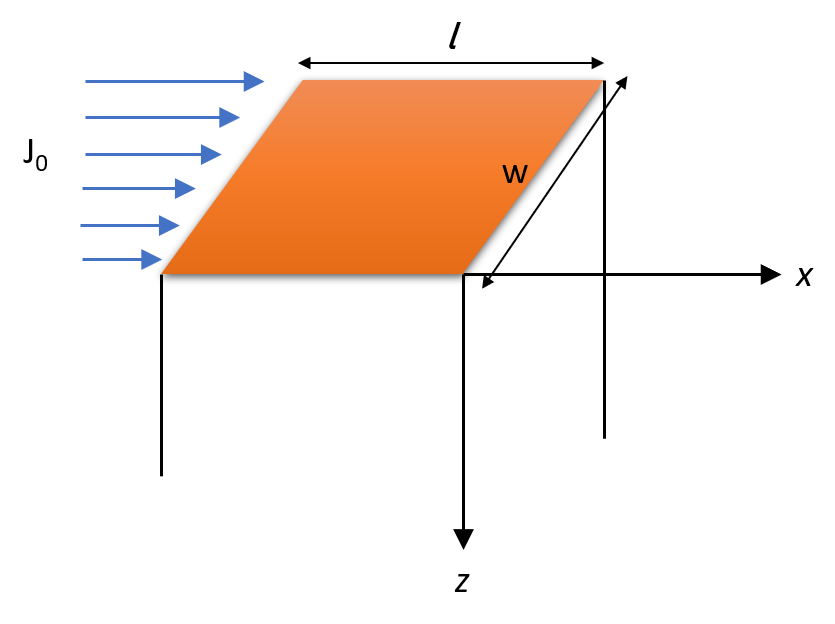
\includegraphics[width=\linewidth]{planecurrent.png}
        \end{figure}
    \end{minipage}%
    \begin{minipage}{0.3\textwidth}
    \begin{align*}
        \text{Current crossing }yz\text{ plane, }\widetilde{I} &= w\int_0^\infty\widetilde{J}_x(z)\ dz\\
        &=w\int_0^\infty J_0e^{-\frac{(1+j)z}{\delta_s}}\ dz\\
        &= \frac{J_0w\delta_s}{1+j}\ \text{(A)}
    \end{align*}
    \end{minipage}
    \item Voltage across length $\ell$ at the surface, $\widetilde{V} = E_0\ell = \displaystyle\frac{J_0}{\sigma}\ell$
    \begin{align*}
        Z &= \frac{\widetilde{V}}{\widetilde{I}} = \frac{1+j}{\sigma\delta_s}\frac{\ell}{w}\\
        &= Z_s\frac{\ell}{w}\ (\Omega)
    \end{align*}
    \newpage
    \item Internal/surface impedance of conductor, $Z_s$
    \begin{center}
        \boxed{Z_s = \displaystyle\frac{1+j}{\sigma\delta_s}\ (\Omega)}
    \end{center}
    \begin{itemize}[label=$\circ$]
        \item Defined as impedance $Z$ for a 1 m length $\ell$ and 1 m width $w$
        \item A complex quantity, can be expressed in terms of $R_s$ and $L_s$, where $Z_s = R_s+j\omega L_s$.
        \begin{center}
            \boxed{$$\begin{array}{c}
                 R_s = \displaystyle\frac{1}{\sigma\delta_s} = \sqrt{\displaystyle\frac{\pi f\mu}{\sigma}}\ (\Omega)\\
                 L_s = \displaystyle\frac{1}{\omega\sigma\delta_s} = \displaystyle\frac{1}{2}\sqrt{\displaystyle\frac{\mu}{\pi f\sigma}}\ \text{(H)}
            \end{array}$$}
        \end{center}
        \item Conductor equivalent to resistor in series with inductor
    \end{itemize}
    \item AC resistance of slab of width $w$ and length $\ell$, $R$
    \begin{center}
        \boxed{$$\begin{array}{cc}
            R = R_s\displaystyle\frac{\ell}{w} = \frac{1}{\sigma\delta_s w}\ (\Omega)  
        \end{array}$$}
    \end{center}
\end{itemize}

\subsection{Power Density}
\begin{itemize}
    \item For any wave with $\overrightarrow{E}$ and $\overrightarrow{H}$,
    Poynting vector $\overrightarrow{S} = \overrightarrow{E}\times\overrightarrow{H}\ \text{(W/}\text{m}^2)$.
    \begin{itemize}[label=$\circ$]
        \item Direction of $\overrightarrow{S}$ along direction of wave propagation
        \item $\overrightarrow{S}$: power density (power per unit area) carried by wave
    \end{itemize}
    \item If wave is incident upon aperture of area with outward surface unit vector $\hat{n}$,
    $$\text{Power intercepted by aperture, }P=\int\limits_A \overrightarrow{S}\cdot\hat{n}\ dA\text{ (W)}$$
    \begin{itemize}[label=$\circ$]
        \item For a plane wave propagating in direction $\hat{k}$ that makes an angle $\theta$ with $\hat{n}$,\\
        $P = SA\cos\theta,$ where $S=|\overrightarrow{S}|$.
    \end{itemize}
    \item Average power density of wave, $\overrightarrow{S_\text{av}}$
    $$\overrightarrow{S_\text{av}} = \frac{1}{2}\operatorname{Re}\left[\widetilde{E}\times\widetilde{H}^*\right]\text{ (W/}\text{m}^2)$$
\end{itemize}

\subsection{Power Density in Lossless Medium}
\begin{itemize}
    \item Average power density carried by wave, $\overrightarrow{S_\text{av}}$
    \begin{center}
        \boxed{$$\begin{array}{ccl}
            \overrightarrow{S_\text{av}} &=&\hat{z}\displaystyle\frac{1}{2\eta}(|E_{x0}|^2+|E_{y0}|^2)  \\[0.4cm]
             &= &\hat{z}\displaystyle\frac{|\widetilde{E}|^2}{2\eta}\text{ (W/}\text{m}^2)
        \end{array}$$}
    \end{center}
\end{itemize}
\subsection{Power Density in Lossy Media}
\begin{itemize}
    \item Average power density carried by wave, $\overrightarrow{S_\text{av}}$
    \begin{center}
        \boxed{$$\begin{array}{ccl}
            \overrightarrow{S_\text{av}} &= &\displaystyle\frac{1}{2}\operatorname{Re}\left[\widetilde{E}\times\widetilde{H}^*\right]\\[0.4cm]
             &= &\displaystyle\frac{\hat{z}(|E_{x0}|^2+|E_{y0}|^2)}{2}e^{-2\alpha z}\operatorname{Re}\left(\frac{1}{\eta_c^*}\right)\text{ (W/}\text{m}^2)
        \end{array}$$}
    \end{center}
    \begin{itemize}[label=$\circ$]
        \item Express $\eta_c$ in polar form, where $\eta_c = |\eta_c|e^{j\theta\eta}$:
        \begin{center}
            \boxed{\overrightarrow{S_\text{av}}(z) = \hat{z}\frac{|\widetilde{E}(0)|^2}{2|\eta_c|}e^{-2\alpha z}\cos\theta_\eta\text{ (W/}\text{m}^2)}
        \end{center}
        \item While $\widetilde{E}(z)$ and $\widetilde{H}(z)$ decay with $z$ as $e^{-\alpha z}$, power density $\overrightarrow{S_\text{av}}$ decreases as $e^{-2\alpha z}$.
    \end{itemize}
\end{itemize}

\subsection{Attenuation Rate}
\begin{itemize}
    \item Attenuation rate, $A$: rate of decrease of magnitude of $\overrightarrow{S_\text{av}}(z)$ as a function of propagation distance
    \begin{align*}
        A &= 10\log\left[\frac{S_\text{av}(z)}{S_\text{av}(0)}\right]\\
        &= 10\log(e^{-2\alpha z})\\
        &= -20\alpha z\log e\\
        &= -8.68\alpha z
    \end{align*}
    \begin{itemize}[label=$\circ$]
        \item where $\alpha$ [dB/m] = $8.68\alpha$ [Np/m]
    \end{itemize}
\end{itemize}

\newpage
\section{W11: Boundary Conditions}
\begin{itemize}
    \item Wave reflection and transmission can be divided into two types: normal and oblique incidences
\end{itemize}

\subsection{Waves at Normal Incidence}
\begin{itemize}
    \item Wave crosses planar boundaries at an angle of $90^\circ$
    \item Assuming:
    \begin{itemize}[label=$\circ$]
        \item Planar boundary at $z=0$,
        \item Electric field propagates in positive $x$-direction,
        \item Magnetic field propagates in positive $z$-direction.
    \end{itemize}
    \item Incident waves
    \begin{itemize}[label=$\circ$]
        \item Incident electric field, $\widetilde{E}^i(z) = \hat{x}E_{0}^ie^{-jk_1z}$
        \item Incident magnetic field, $\widetilde{H}^i(z) = \hat{z}\times\displaystyle\frac{\widetilde{E}^i_0(z)}{\eta_1} = \hat{y}\displaystyle\frac{\widetilde{E}^i(z)}{\eta_1} = \hat{y}\displaystyle\frac{E^i_0}{\eta_1}e^{-jk_1z}$
    \end{itemize}
    \item Reflected waves
    \begin{itemize}[label=$\circ$]
        \item Reflected electric field, $\widetilde{E}^r(z) = \hat{x}E^r_0e^{jk_1z}$
        \item Reflected magnetic field, $\widetilde{H}^r(z) = \hat{z}\times\displaystyle\frac{\widetilde{E}_r(z)}{\eta_1} = -\hat{y}\displaystyle\frac{E^r_0}{\eta_1}e^{jk_1z}$
    \end{itemize}
    \item Transmitted waves
    \begin{itemize}[label=$\circ$]
        \item Transmitted electric field, $\widetilde{E}^t(z) = \hat{x}E^t_0e^{-jk_2z}$
        \item Transmitted magnetic field, $\widetilde{H}^t(z) = \hat{z}\times\displaystyle\frac{\widetilde{E}^t(z)}{\eta_2} = \hat{y}\displaystyle\frac{E^t_0}{\eta_2}e^{-jk_2z}$
    \end{itemize}
    \item Waves in Medium 1
    \begin{itemize}[label=$\circ$]
        \item Total electric field in Medium 1, $\widetilde{E}_1(z) = \widetilde{E}^i(z) + \widetilde{E}^r(z) = \hat{x}(E^i_0e^{-jk_1z}+E^r_0e^{jk_1z})$
        \item Total magnetic field in Medium 1, $\widetilde{H}_1(z) = \widetilde{H}^i(z) + \widetilde{H}^r(z) = \hat{y}\displaystyle\frac{1}{\eta_1}(E^i_0e^{-jk_1z}-E^r_0e^{jk_1z})$
    \end{itemize}
    \item Waves in Medium 2
    \begin{itemize}[label=$\circ$]
        \item Total electric field in Medium 2, $\widetilde{E}_2(z) = \hat{x}E^t_0e^{-jk_2z}$
        \item Total magnetic field in Medium 2, $\widetilde{H}_2(z) = \hat{y}\displaystyle\frac{E^t_0}{\eta_2}e^{-jk_2z}$
    \end{itemize}
\end{itemize}

\newpage
\subsection{Boundary Conditions}
\begin{itemize}
    \item At the boundary $z = 0$:
    \begin{align*}
        \widetilde{E}_1(0) &= \widetilde{E}_2(0)\quad \text{ or }\quad E^i_0+E^r_0=E^t_0\\
        \widetilde{H}_1(0) &= \widetilde{H}_2(0)\quad \text{ or } \quad \displaystyle\frac{E^i_0}{\eta_1}-\displaystyle\frac{E^r_0}{\eta_1} = \displaystyle\frac{E^t_0}{\eta_2}
    \end{align*}
    \item Solving the above set of equations gives:
    \begin{align*}
        E^r_0 &= \left(\frac{\eta_2-\eta_1}{\eta_2+\eta_1}\right)E^i_0 = \Gamma E^i_0\\
        E^t_0 &= \left(\frac{2\eta_2}{\eta_2+\eta_1}\right)E^i_0 = \tau E^i_0
    \end{align*}
    \item Reflection coefficient, $\Gamma = \displaystyle\frac{E^r_0}{E^i_0} = \frac{\eta_2-\eta_1}{\eta_2+\eta_1}\quad\text{(normal incidence)}$
    \item Transmission coefficient, $\tau = \displaystyle\frac{E^t_0}{E^i_0} = \displaystyle\frac{2\eta_2}{\eta_2+\eta_1}\quad\text{(normal incidence)}$
    \item $\Gamma$ and $\tau$ are related: $\tau = 1+\Gamma\quad\text{(normal incidence)}$
    \item For non-magnetic media, $\eta_1 = \displaystyle\frac{\eta_0}{\sqrt{\epsilon_{r1}}},\ \eta_2 = \displaystyle\frac{\eta_0}{\sqrt{\epsilon_{r2}}}$ where $\eta_0$ is the intrinsic impedance of free space.
    $$\Rightarrow \Gamma = \frac{\sqrt{\epsilon_{r1}}-\sqrt{\epsilon_{r2}}}{\sqrt{\epsilon_{r1}}+\sqrt{\epsilon_{r2}}}\quad\text{(non-magnetic media)}$$
\end{itemize}

\subsection{Snell's Law}
\begin{itemize}
    \item Angles measured with respect to normal of planar boundaries:
    \begin{itemize}[label=$\circ$]
        \item $\theta_i$: Angle of incidence
        \item $\theta_r$: Angle of reflection
        \item $\theta_t$: Angle of transmission
    \end{itemize}
    \begin{center}
        \boxed{\begin{array}{cl}
             \text{Snell's Law of Reflection} & \theta_i = \theta_r \\
             \text{Snell's Law of Refraction} & \displaystyle\frac{\sin\theta_t}{\sin\theta_i} = \displaystyle\frac{u_{p1}}{u_{p2}} = \sqrt{\displaystyle\frac{\mu_1\epsilon_1}{\mu_2\epsilon_2}}
        \end{array}}
    \end{center}
    \item For non-magnetic materials, $\displaystyle\frac{\sin\theta_1}{\sin\theta_2} = \frac{n_1}{n_2} = \sqrt{\frac{\epsilon_{r1}}{\epsilon_{r2}}}$.
\end{itemize}

\newpage
\subsection{Refraction Index}
\begin{itemize}
    \item Refraction index: ratio of phase velocity in free space to phase velocity in a particular medium
    $$n = \frac{c}{u_p} = \sqrt{\frac{\mu\epsilon}{\mu_0\epsilon_0}} = \sqrt{\mu_r\epsilon_r}$$
    \item A material is referred as more dense than another material if it has a greater index of refraction.
\end{itemize}

\subsection{Critical Angle \& Total Internal Reflection}
\begin{itemize}
    \item Critical angle: angle of incidence when $\theta_t=90^\circ$
    $$\sin\theta_c = \left.\frac{n_2}{n_1}\sin\theta_t\right|_{\theta_t = 90^\circ}= \frac{n_2}{n_1}$$
    \item For non-magnetic materials, $\mu_1 = \mu_2$:
    $$\Rightarrow\sin\theta_c = \sqrt{\frac{\epsilon_{r2}}{\epsilon_{r1}}}$$
    \item When $\theta_i>\theta_c$, total internal reflection occurs.
\end{itemize}

\subsection{Optical Fibre \& Modal Dispersion}
\begin{itemize}
    \item Acceptance angle, $\theta_a$: maximum value of $\theta_i$ for which total internal reflection remains satisfied
    $$\sin\theta_a = \frac{1}{n_0}(n_f^2-n_c^2)^{1/2}$$
    \begin{itemize}[label=$\circ$]
        \item where $n_f$ is the refraction index of the fibre core,
        \item $n_c$ is the refraction index of cladding,
        \item and $n_0$ is the refraction index of air.
    \end{itemize}
    \item Optical fibres have a property called \textbf{modal dispersion}, which causes the distortion of the shape of transmitted pulses of digital data.
    $$\text{Highest data rate, }f_p = \frac{1}{T} = \frac{1}{2\tau} = \frac{cn_c}{2\ell n_f(n_f-n_c)}\quad\text{ (bits/s)}$$
\end{itemize}


\subsection{Plane of Incidence}
\begin{itemize}
    \item Plane of incidence: plane which contains normal to boundary and direction of propagation of incident wave
\end{itemize}

\subsection{Perpendicular Polarization (TE Waves)}
\begin{itemize}
    \item Incident electric field $\widetilde{E}^i$ is perpendicular to plane of incidence
    \item Also known as transverse electric waves (TE waves)
    \item Incident waves
    \begin{itemize}[label=$\circ$]
        \item Incident electric field, $\widetilde{E}^i_\perp = \hat{y}E^i_\perp e^{-jk_1x_i} = \hat{y}E^i_{\perp 0} e^{-jk_1(x\sin\theta_i+z\cos\theta_i)}$
        \item Incident magnetic field, $\widetilde{H}^i_\perp = (-\hat{x}\cos\theta_i+\hat{z}\cos\theta_i)\times\displaystyle\frac{E^i_{\perp 0}}{\eta_1}e^{-jk_1(x\sin\theta_i+z\cos\theta_i)}$
    \end{itemize}
    \item Reflected waves
    \begin{itemize}[label=$\circ$]
        \item Reflected electric field, $\widetilde{E}^r_\perp = \hat{y}E^r_{\perp 0}e^{-jk_1x_r} = \hat{y}E^r_{\perp 0}e^{-jk_1(x\sin\theta_r-z\cos\theta_r)}$
        \item Reflected magnetic field, $\widetilde{H}^r_\perp = (\hat{x}\cos\theta_r+\hat{z}\sin\theta_r)\times\displaystyle\frac{E^r_{\perp 0}}{\eta_1}e^{-jk_1(x\sin\theta_r - z\cos\theta_r)}$
    \end{itemize}
    \item Transmitted waves
    \begin{itemize}[label=$\circ$]
        \item Transmitted electric field, $\widetilde{E}^t_\perp = \hat{y}E^t_{\perp 0}e^{-jk_2x_t} = \hat{y}E^t_{\perp 0}e^{-jk_2(x\sin\theta_t+z\cos\theta_t)}$
        \item Transmitted magnetic field, $\widetilde{H}^t_\perp = (-\hat{x}\cos\theta_t+\hat{z}\sin\theta_t)\times\displaystyle\frac{E^t_{\perp 0}}{\eta_2}e^{-jk_2(x\sin\theta_t+z\cos\theta_t)}$
    \end{itemize}
    \item Tangential electric field continuous boundary conditions
    \begin{align*}
        \left.(\widetilde{E}^i_{\perp y}+\widetilde{E}^r_{\perp y})\right|_{z=0} &= \left.\widetilde{E}^t_{\perp y}\right|_{z=0}\\
        E^i_{\perp 0}e^{-jk_1 x\sin\theta_i} + E^r_{\perp 0}e^{-jk_1 x\sin\theta_r} &= E^t_{\perp 0}e^{-jk_2\sin\theta_t}
    \end{align*}
    \item Tangential magnetic field continuous boundary conditions
    \begin{align*}
        \left.(\widetilde{H}^i_{\perp x}+\widetilde{H}^r_{\perp x})\right|_{z=0} &= \left.\widetilde{H}^t_{\perp x}\right|_{z=0}\\
        -\frac{E^i_{\perp 0}}{\eta_1}\cos\theta_i e^{-jk_1 x\sin\theta_i} + \frac{E^r_{\perp 0}}{\eta_1}\cos\theta_r e^{-jk_1 x\sin\theta_r} &= -\frac{E^t_{\perp 0}}{\eta_2}\cos\theta_t e^{-jk_2\sin\theta_t}
    \end{align*}
    \item Solutions of boundary equations
    \begin{enumerate}
        \item Exponents are equal for all values of $x$.
        $$k_1\sin\theta_i = k_1\sin\theta_r = k_2\sin\theta_t$$
        \item For the remaining terms:
        \begin{center}
            $\begin{array}{c}
                 E^i_{\perp 0} + E^r_{\perp 0} = E^t_{\perp 0}\\
                 \Rightarrow \displaystyle\frac{\cos\theta_i}{\eta_1}(-E^i_{\perp 0}+E^r_{\perp 0}) = -\displaystyle\frac{\cos\theta_t}{\eta_2}E^t_{\perp 0} 
            \end{array}$
        \end{center}
    \end{enumerate}
\end{itemize}

\subsection{Fresnel Reflection and Transmission Coefficients for TE Waves}
\begin{itemize}
    \item Reflection coefficient, $\Gamma_\perp = \displaystyle\frac{E^r_{\perp 0}}{E^i_{\perp 0}} = \displaystyle\frac{\eta_2\cos\theta_i-\eta_1\cos\theta_t}{\eta_2\cos\theta_i+\eta_1\cos\theta_t}$
    \item Transmission coefficient, $\tau_\perp = \displaystyle\frac{E^t_{\perp 0}}{E^i_{\perp 0}} = \displaystyle\frac{2\eta_2\cos\theta_i}{\eta_2\cos\theta_i+\eta_1\cos\theta_t}$
    \item $\Gamma_\perp$ and $\tau_\perp$ are related: $\tau_\perp = 1+\Gamma_\perp$
    \item For non-magnetic dielectrics, $\mu_1 = \mu_2 = \mu_0$:
    $$\Rightarrow \Gamma_\perp = \frac{\cos\theta_i-\sqrt{\displaystyle\frac{\epsilon_2}{\epsilon_1}-\sin^2\theta_i}}{\cos\theta_i+\sqrt{\displaystyle\frac{\epsilon_2}{\epsilon_1}-\sin^2\theta_i}}$$
\end{itemize}

\subsection{Parallel Polarization (TM Waves)}
\begin{itemize}
    \item Incident electric field $\widetilde{E}^i$ is parallel to plane of incidence
    \item Also known as transverse magnetic waves (TM waves)
    \item Incident waves
    \begin{itemize}[label=$\circ$]
        \item Incident electric field, $\widetilde{E}^i_\parallel$
        \begin{align*}
           \widetilde{E}^i_\parallel &= (\hat{x}\cos\theta_i -\hat{z}\sin\theta_i)E^i_{\parallel 0} e^{-jk_1x_i}\\
           &= (\hat{x}\cos\theta_i -\hat{z}\sin\theta_i)E^i_{\parallel 0} e^{-jk_1(x\sin\theta_i+z\cos\theta_i)} 
        \end{align*}
        \item Incident magnetic field, $\widetilde{H}^i_\parallel = \hat{y}\displaystyle\frac{E^i_{\parallel 0}}{\eta_1}e^{-jk_1(x\sin\theta_i+z\cos\theta_i)}$
    \end{itemize}
    \item Reflected waves
    \begin{itemize}[label=$\circ$]
        \item Reflected electric field, $\widetilde{E}^r_\parallel$
        \begin{align*}
            \widetilde{E}^r_\parallel &= (\hat{x}\cos\theta_r +\hat{z}\sin\theta_i)E^r_{\parallel 0} e^{-jk_1x_r}\\
            &= (\hat{x}\cos\theta_r +\hat{z}\sin\theta_i)E^r_{\parallel 0} e^{-jk_1(x\sin\theta_r-z\cos\theta_r)}
        \end{align*}
        \item Reflected magnetic field, $\widetilde{H}^r_\perp = -\hat{y}\displaystyle\frac{E^r_{\parallel 0}}{\eta_1}e^{-jk_1(x\sin\theta_r-z\cos\theta_r)}$
    \end{itemize}
    \item Transmitted waves
    \begin{itemize}[label=$\circ$]
        \item Transmitted electric field, $\widetilde{E}^t_\parallel$
        \begin{align*}
            \widetilde{E}^t_\parallel &= (\hat{x}\cos\theta_t-\hat{z}\sin\theta_t)E^t_{\parallel 0}e^{-jk_2x_t}\\
            &= (\hat{x}\cos\theta_t-\hat{z}\sin\theta_t)E^t_{\parallel 0}e^{-jk_2(x\sin\theta_t+z\cos\theta_t)}
        \end{align*}
        \item Transmitted magnetic field, $\widetilde{H}^t_\parallel = \hat{y}\displaystyle\frac{E^t_{\parallel 0}}{\eta_2}e^{-jk_2(x\sin\theta_t+z\cos\theta_t)}$
    \end{itemize}
\end{itemize}

\subsection{Fresnel Reflection and Transmission Coefficients for TM Waves}
\begin{itemize}
    \item Reflection coefficient, $\Gamma_\parallel = \displaystyle\frac{E^r_{\parallel 0}}{E^i_{\parallel 0}} = \displaystyle\frac{\eta_2\cos\theta_t-\eta_1\cos\theta_t}{\eta_2\cos\theta_t+\eta_1\cos\theta_t}$
    \item Transmission coefficient, $\tau_\parallel = \displaystyle\frac{E^t_{\parallel 0}}{E^i_{\parallel 0}} = \displaystyle\frac{2\eta_2\cos\theta_i}{\eta_2\cos\theta_t+\eta_1\cos\theta_t}$
    \item $\Gamma_\parallel$ and $\tau_\parallel$ are related: $\tau_\parallel = (1+\Gamma_\parallel)\displaystyle\frac{\cos\theta_i}{\cos\theta_t}$
    \item For non-magnetic dielectrics, $\mu_1 = \mu_2 = \mu_0$:
    $$\Rightarrow \Gamma_\parallel = \displaystyle\frac{-\displaystyle\frac{\epsilon_2}{\epsilon_1}\cos\theta_i+\sqrt{\displaystyle\frac{\epsilon_2}{\epsilon_1}-\sin^2\theta_i}}{\displaystyle\frac{\epsilon_2}{\epsilon_1}\cos\theta_i+\sqrt{\displaystyle\frac{\epsilon_2}{\epsilon_1}-\sin^2\theta_i}}$$
\end{itemize}

\subsection{Brewster Angle}
\begin{itemize}
    \item The incidence angle $\theta_i$ at which the Fresnel reflection coefficient $\Gamma = 0$
    \item Does not exist for non-magnetic materials in perpendicular polarization (TE wave)
    \item In parallel polarization for $\mu_1 = \mu_2$:
    \begin{align*}
        \theta_{B \parallel} &= \sin^{-1}\sqrt{\frac{1}{1+\displaystyle\frac{\epsilon_1}{\epsilon_2}}}\\
        &= \tan^{-1}\sqrt{\displaystyle\frac{\epsilon_2}{\epsilon_1}}
    \end{align*}
\end{itemize}

\subsection{Reflectivity and Transmittivity}
\begin{itemize}
    \item Reflectivity: ratio of reflected power to incident power
    \begin{align*}
        R_\perp &= |\Gamma_\perp|^2 = \frac{P^r_\perp}{P^i_\perp}\\
        R_\parallel &= |\Gamma_\parallel|^2 = \frac{P^r_\parallel}{P^i_\parallel}
    \end{align*}
    \item Transmittivity: ratio of transmitted power to incident power
    \begin{align*}
        T_\perp &= \frac{P^t_\perp}{P^i_\perp} = |\tau_\perp|^2\left(\frac{\eta_1\cos\theta_t}{\eta_2\cos\theta_i}\right)\\
        T_\parallel &= \frac{P^t_\parallel}{P^i_\parallel} = |\tau_\parallel|^2\left(\frac{\eta_1\cos\theta_t}{\eta_2\cos\theta_i}\right)
    \end{align*}
    \item Reflectivity is related to transmittivity:
    \begin{align*}
        R_\perp + T_\perp &= 1\\
        R_\parallel + T_\parallel &= 1
    \end{align*}
\end{itemize}

\newpage
\section{W12: Waveguides and Resonators}

\subsection{Waveguides}
\begin{itemize}
    \item Carries energy by non-TEM modes such as TE and TM modes or combination of both
    \begin{itemize}[label=$\circ$]
        \item TE mode: when $\widetilde{E}$ is transverse to $\hat{k}$ but $\widetilde{H}$ is not
        \item TM mode: when $\widetilde{H}$ is transverse to $\hat{k}$ but $\widetilde{E}$ is not
    \end{itemize}
    \item e.g. optical fiber, metal waveguides
    \item Inner conduction of coaxial cable can couple energy from and into waveguide
\end{itemize}

\subsection{Transverse Magnetic (TM) Mode}
\begin{itemize}
    \item Boundary conditions:
    $$k_x = \frac{m\pi}{a},\ m=1, 2, 3,\ldots\quad\text{ and }\quad k_y = \frac{n\pi}{b},\ n=1, 2, 3,\ldots\quad\text{where }k_c^2 = k_x^2+k_y^2$$
    \begin{itemize}[label=$\circ$]
        \item Cutoff wave number, $k_c = k^2-\beta^2 = \omega^2\mu\epsilon-\beta^2$
    \end{itemize}
    \item For a wave propagating in $z$-direction with $\widetilde{H}_z = 0$:
    \begin{itemize}[label=$\circ$]
        \item $\widetilde{E}_x = -\displaystyle\frac{j\beta}{k_c^2}\left(\displaystyle\frac{m\pi}{a}\right)E_0\cos\left(\displaystyle\frac{m\pi x}{a}\right)\sin\left(\displaystyle\frac{n\pi y}{b}\right)e^{-j\beta z}$
        \item $\widetilde{E}_y = -\displaystyle\frac{j\beta}{k_c^2}\left(\displaystyle\frac{n\pi}{b}\right)E_0\sin\left(\displaystyle\frac{m\pi x}{a}\right)\cos\left(\displaystyle\frac{n\pi y}{b}\right)e^{-j\beta z}$
        \item $\widetilde{E}_z = E_0\sin\left(\displaystyle\frac{m\pi x}{a}\right)\sin\left(\displaystyle\frac{n\pi y}{b}\right)e^{-j\beta z}$
        \item $\widetilde{H}_x = \displaystyle\frac{j\omega\epsilon}{k_c^2}\left(\displaystyle\frac{n\pi}{b}\right)E_0\sin\left(\displaystyle\frac{m\pi x}{a}\right)\cos\left(\displaystyle\frac{n\pi y}{b}\right)e^{-j\beta z}$
        \item $\widetilde{H}_y = - \displaystyle\frac{j\omega\epsilon}{k_c^2}\left(\displaystyle\frac{m\pi}{a}\right)E_0\cos\left(\displaystyle\frac{m\pi x}{a}\right)\sin\left(\displaystyle\frac{n\pi y}{b}\right)e^{-j\beta z}$
    \end{itemize}
    \item $m$ and $n$ are positive integers
    \item Each combination of $m$ and $n$ represents a mode, denoted as $\text{TM}_\text{mn}$.
\end{itemize}

\newpage
\subsection{Transverse Electric (TE) Mode}
\begin{itemize}
    \item Boundary conditions:
    $$k_x = \frac{m\pi}{a},\ m=1, 2, 3,\ldots\quad\text{ and }\quad k_y = \frac{n\pi}{b},\ n=1, 2, 3,\ldots\quad\text{where }k_c^2 = k_x^2+k_y^2$$
    \begin{itemize}[label=$\circ$]
        \item Cutoff wave number, $k_c = k^2-\beta^2 = \omega^2\mu\epsilon-\beta^2$
    \end{itemize}
    \item For a wave propagating in $z$-direction with $\widetilde{E}_z = 0$:
    \begin{itemize}[label=$\circ$]
        \item $\widetilde{E}_x =  \displaystyle\frac{j\omega\mu}{k_c^2}\left(\displaystyle\frac{n\pi}{b}\right)H_0\cos\left(\displaystyle\frac{m\pi x}{a}\right)\sin\left(\displaystyle\frac{n\pi y}{b}\right)e^{-j\beta z}$
        \item $\widetilde{E}_y = - \displaystyle\frac{j\omega\mu}{k_c^2}\left(\displaystyle\frac{m\pi}{a}\right)H_0\sin\left(\displaystyle\frac{m\pi x}{a}\right)\cos\left(\displaystyle\frac{n\pi y}{b}\right)e^{-j\beta z}$
        \item $\widetilde{H}_x = \displaystyle\frac{j\beta}{k_c^2}\left(\displaystyle\frac{m\pi}{a}\right)H_0\sin\left(\displaystyle\frac{m\pi x}{a}\right)\cos\left(\displaystyle\frac{n\pi y}{b}\right)e^{-j\beta z}$
        \item $\widetilde{H}_y = \displaystyle\frac{j\beta}{k_c^2}\left(\displaystyle\frac{n\pi}{b}\right)H_0\cos\left(\displaystyle\frac{m\pi x}{a}\right)\sin\left(\displaystyle\frac{n\pi y}{b}\right)e^{-j\beta z}$
        \item $\widetilde{H}_z = H_0\cos\left(\displaystyle\frac{m\pi x}{a}\right)\cos\left(\displaystyle\frac{n\pi y}{b}\right)e^{-j\beta z}$
    \end{itemize}
    \item $m$ and $n$ are positive integers
    \item Each combination of $m$ and $n$ represents a mode, denoted as $\text{TE}_\text{mn}$.
\end{itemize}

\subsection{Properties of TM and TE Modes}
\begin{itemize}
    \item Phase constant, $\beta$
    \begin{align*}
        \beta &= \sqrt{k^2-k_c^2}\\
        &= \sqrt{\omega^2\mu\epsilon-\left(\frac{m\pi}{a}\right)^2-\left(\frac{n\pi}{b}\right)^2}\quad\text{(TE and TM)}
    \end{align*}
    \item Cutoff frequency, $f_{mn}$
    \begin{align*}
        f_{mn} = \frac{u_\text{p0}}{2}\sqrt{\left(\frac{m}{a}\right)^2+\left(\frac{n}{b}\right)^2}\quad\text{(TE and TM)}
    \end{align*}
    \begin{itemize}[label=$\circ$]
        \item Frequency at each mode $mn$ when $\beta = 0$
        \item Value of 0 for m or n is NOT allowed for TM modes
        \item A wave can propagate through waveguide if and only if $f > f_{mn}$
    \end{itemize}
    \item Wave impedance in TM mode of waveguide, $Z_\text{TM}$
    \begin{align*}
        Z_\text{TM} &= \frac{\widetilde{E}_x}{\widetilde{H}_y} = -\frac{\widetilde{E}_y}{\widetilde{H}_x} = \frac{\beta\eta}{k}\\
        &= \eta\sqrt{1-\left(\frac{f_{mn}}{f}\right)^2}
    \end{align*}
    \item Wave impedance in TE mode of waveguide, $Z_\text{TE}$
    \begin{align*}
        Z_\text{TM} &= \frac{\widetilde{E}_x}{\widetilde{H}_y} = -\frac{\widetilde{E}_y}{\widetilde{H}_x}\\
        &= \frac{\eta}{\sqrt{1-\left(\displaystyle\frac{f_{mn}}{f}\right)^2}}
    \end{align*}
\end{itemize}

\subsection{Propagation Velocities}
\begin{itemize}
    \item Phase velocity, $u_p$: velocity of sinusoidal pattern of wave
    \begin{align*}
        u_p = \frac{\omega}{\beta} = \frac{u_\text{p0}}{\sqrt{1-\left(\displaystyle\frac{f_{mn}}{f}\right)^2}}\quad\text{(TE and TM)}
    \end{align*}
    \item Group velocity, $u_g$: velocity of envelope or wave group travelling through the medium
    $$u_g = \frac{d\omega}{d\beta   } = u_\text{p0}\sqrt{1-\left(\frac{f_{mn}}{f}\right)^2}$$
\end{itemize}

\subsection{\texorpdfstring{$\omega$-$\beta$}{Omega-Beta}  Diagram}
\begin{itemize}
    \item Phase velocity $u_p$: ratio of $\omega$ to $\beta$
    \item Group velocity $u_g$: slope $\displaystyle\frac{d\omega}{d\beta}$ of the curve 
    \item As $f\gg f_{mn}$, $\omega$-$\beta$ curve approaches TEM case where $u_p=u_g$.
    \item $u_p$ and $u_g$ are related by the following equation: \quad $u_pu_g = u_\text{p0}^2$
\end{itemize}

\subsection{Zigzag Reflections}
\begin{itemize}
    \item $\text{TE}_{101}$ can be constructed as sum of two TEM waves
\end{itemize}

\subsection{Resonant Cavities}
\begin{itemize}
    \item Cavities have metal walls on all 6 sides, unlike waveguides which only have 4 conducting sides
    \item Can be used as circuit elements in microwave oscillators, amplifiers and bandpass filters
    \item Resonant frequency, $f_{mnp} = \displaystyle\frac{u_{p0}}{2}\sqrt{\left(\displaystyle\frac{m}{a}\right)^2+\left(\displaystyle\frac{n}{b}\right)^2+\left(\displaystyle\frac{p}{d}\right)^2}$
    \begin{itemize}[label=$\circ$]
        \item For TE mode, $m$ and $n$ start at 0 while $p$ starts at 1.
        \item For TM mode, $m$ and $n$ start at 1 while $p$ starts at 0.
    \end{itemize}
    \item Quality factor, $Q$: approximately equivalent to normalized bandwidth
    $$Q \approx \frac{f_{mnp}}{\Delta f}$$
    \begin{itemize}[label=$\circ$]
        \item In $\text{TE}_{101}$ mode, $Q = \displaystyle\frac{1}{\delta_s}\displaystyle\frac{abd(a^2+d^2)}{[a^3(d+2b)+d^3(a+2b)]}$,
        \begin{itemize}[label=\tiny$\blacksquare$]
            \item where skin depth $\delta_s = \displaystyle\frac{1}{\sqrt{\pi f_{mnp}\mu_0\sigma_c}}$,
            \item and $\sigma_c$ is the electrical conductivity of the conducting walls.
        \end{itemize}
    \end{itemize}
\end{itemize}

\newpage
\section{W13: Antennas II}

\subsection{Normalized Radiation Intensity}
\begin{itemize}
    \item Electric field, $\widetilde{E}_\theta = \displaystyle\frac{jI_0\ell k\eta_0}{4\pi}\left(\displaystyle\frac{e^{-jkR}}{R}\right)\sin\theta\quad\text{(V/m)}$
    \item Magnetic field, $\widetilde{H}_\phi = \displaystyle\frac{\widetilde{E}_\theta}{\eta_0}\quad\text{(A/m)}$ 
    \item Average power density, $\overrightarrow{S_\text{av}} = \hat{R}\ S(R, \theta) = \displaystyle\frac{1}{2}\operatorname{Re}\left[\widetilde{E}\times\widetilde{H}^*\right]\quad\text{(W/}\text{m}^2)$
    \item Power density, $S(R, \theta)$
    \begin{align*}
        S(R, \theta) &= \left(\displaystyle\frac{\eta_0k^2I_0\ell^2}{32\pi^2R^2}\right)\sin^2\theta\\
        &= S_0\sin^2\theta\quad\text{(W/}\text{m}^2)
    \end{align*}
    \item Maximum power density, $S_\text{max}$
    \begin{align*}
        S_\text{max} &= S_0 = \frac{\eta_0k^2I_0\ell^2}{32\pi^2R^2}\\
        &= \frac{15\pi I_0^2}{R^2}\left(\frac{\ell}{\pi}\right)^2\quad\text{(W/}\text{m}^2)
    \end{align*}
    \item Normalized radiation intensity, $F(\theta, \phi)$:
    \begin{align*}
        F(\theta, \phi) = \frac{S(R, \theta, \phi)}{S_\text{max}}\quad\text{(dimensionless)}
    \end{align*}
\end{itemize}

\subsection{Reciprocity}
\begin{itemize}
    \item Receiving antenna has same directional antnna pattern as transmitting antenna.
\end{itemize}

\subsection{Total Radiation Power}
\begin{itemize}
    \item Total radiation power, $P_\text{rad}$
    \begin{align*}
        P_rad &= R^2\int^{2\pi}_{\phi=0^\circ}\int^\pi_{\theta=0^\circ}S(R,\theta,\phi)\sin\theta\ d\theta\ d\phi\\
        &= R^2S_\text{max}\int^{2\pi}_0\int^\pi_0 F(\theta, \phi)\sin\theta\ d\theta\ d\phi\\
        &= R^2S_\text{max}\iint\limits_{4\pi}F(\theta, \phi)\ d\Omega\quad\text{(W)}
    \end{align*}
\end{itemize}

\newpage
\subsection{Antenna Patterns}
\begin{itemize}
    \item Two principal planes:
    \begin{enumerate}
        \item Elevation plane ($xz$ and $yz$ planes): constant value of $\phi$
        \item Azimuth plane ($xy$ plane): $\theta = 90^\circ$
    \end{enumerate}
    \item 2D pattern:
    \begin{itemize}[label=$\circ$]
        \item Main lobe: where most energy is radiated
        \item Side lobe: where some energy is radiated
        \item Back lobe: opposite to main lobe
    \end{itemize}
\end{itemize}

\subsection{Pattern Solid Angle}
\begin{itemize}
    \item Pattern solid angle, $\Omega_p$: integral of normalized radiation intensity $F(\theta, \phi)$ over a sphere
    \item Characterizes directional properties of 3D radiation pattern
    $$\Omega_p = \iint\limits_{4\pi}F(\theta, \phi)\ d\Omega\text{ (sr)}$$
    \item For isotropic antennas, $F(\theta, \phi) = 1 \Rightarrow \Omega_p = 4\pi\text{ (sr)}$
\end{itemize}

\subsection{Half Power Beamwidth (HPBW)}
\begin{itemize}
    \item Half power beamwidth, $\beta$: angular width of main lobe between two angles at which magnitude of $F(\theta, \phi)$ is equal to half its peak value
    $$\beta = \phi_2-\phi_1$$
    \begin{itemize}[label=$\circ$]
        \item where $\theta_1$ and $\theta_2$ are the half-power angles at which $F(\theta, \phi) = 0.5F_\text{max}$.
    \end{itemize}
    \item Characterizes directional properties of 2D radiation pattern
    \item Also known as the 3 dB beamwidth since 0.5 corresponds to -3 dB
\end{itemize}

\newpage
\subsection{Directivity}
\begin{itemize}
    \item Directivity: ratio of maximum normal radiation intensity $F_\text{max}$ to average value of $F(\theta, \phi)$ over all directions
    \begin{align*}
        D &= \frac{{F_\text{max}}}{F_\text{av}}\\
        &= \frac{1}{\displaystyle\frac{1}{4\pi}\iint\limits_{4\pi}F(\theta, \phi)\ d\Omega}\\
        &= \frac{4\pi}{\Omega_p}\text{ (dimensionless)}
    \end{align*}
    \item Directivity $\uparrow$, $\Omega_p$ of antenna pattern $\downarrow$
    \item For isotropic antennas, $\Omega_p = 4\pi \Rightarrow D=\displaystyle\frac{4\pi}{4\pi} = 1$
    \item For antenna with single main lobe in $z$-direction, $\Omega_p \approx \beta_{xz}\ \beta_{yz}$
    \begin{itemize}[label=$\circ$]
        \item where $\beta_{xz}$ and $\beta_{yz}$ are the half power beamwidths in radians.
    \end{itemize}
    $$D = \frac{4\pi}{\Omega_p}\approx\frac{4\pi}{\beta_{xz}\ \beta_{yz}}$$
\end{itemize}

\subsection{Radiation Efficiency}
$$\text{Radiation efficiency, }\xi = \frac{P_\text{rad}}{P_\text{t}}\quad\text{(dimensionless)}$$
\begin{itemize}
    \item where $P_\text{rad}$ is the radiated power,
    \item and $P_\text{t}$ is the transmitter power.
\end{itemize}

\subsection{Antenna Gain}
\begin{itemize}
    \item Antenna gain, $G$: accounts for ohmic lossses in antenna material, unlike directivity
    $$G = \xi D\quad\text{(dimensionless)}$$
    \item For a lossless antenna, $\xi = 1\Rightarrow G = D$.
\end{itemize}

\subsection{Effective Area of Antenna}
\begin{itemize}
    \item Effective area, $A_e$: ratio of intercepted power to power density of incident wave
    $$A_e = \frac{P_\text{int}}{S_i}\quad(\text{m}^2)$$
    \item For short dipole antenna, $A_e = \displaystyle\frac{3\lambda^2}{8\pi}\quad(\text{m}^2)$.
    \item For any antenna, $A_e = \displaystyle\frac{\lambda^2 D}{4\pi}\quad(\text{m}^2)$.
\end{itemize}

\subsection{Friis Transmission Formula}
\begin{itemize}
    \item Friis transmission formula:
    \begin{center}
        \boxed{\frac{P_\text{rec}}{P_\text{t}} = \frac{\xi_t\xi_rA_tA_r}{\lambda^2R^2} = G_tG_r\left(\frac{\lambda}{4\pi R}\right)^2,}
    \end{center}
    \begin{itemize}[label = $\circ$]
        \item where $\displaystyle\frac{P_\text{rec}}{P_\text{t}}$ is called the power transfer ratio.
    \end{itemize}
\end{itemize}

\newpage
\appendix
\section{Appendix}
\subsection{Derivatives}
\begin{center}
    $\displaystyle\frac{d}{dt}$\\[0.25cm]
    $\sin\rightarrow\cos,\quad \cos\rightarrow -\sin,\quad \tan\rightarrow\sec^2,\quad x^n\rightarrow nx^{n-1},\quad e^{ax}\rightarrow ae^{ax}, \quad \ln x \rightarrow \displaystyle\frac{1}{x}$
\end{center}
\subsection{Integrals}
\begin{center}
    $\int$\\[0.25cm]
    $\sin\rightarrow -\cos,\quad \cos\rightarrow\sin,\quad \sec^2\rightarrow\tan,\quad x^n\rightarrow\displaystyle\frac{1}{n}x^{n+1},\quad e^{ax}\rightarrow\displaystyle\frac{1}{a}e^{ax},\quad \displaystyle\frac{1}{x}\rightarrow\ln |x|$
\end{center}
\begin{align*}
    \int_0^{\pi/2} \cos^2\theta\sin\theta\ d\theta &= \left[-\frac{\cos^3\theta}{3}\right]_0^{\pi/2} = \frac{1}{3}\\
    \int_0^\pi \sin^3\theta\ d\theta &= \left[\frac{cos^3\theta}{3}-\cos\theta\right]_0^\pi = \frac{4}{3}\\
    \int\sin\theta\cos\theta\ d\theta &= \frac{\sin^2\theta}{2}+C
\end{align*}
\subsection{Integration by Parts}
$$\int u\ dv = uv -\int v du$$
Priority of choosing $u$:
\begin{enumerate}
    \item Logarithmic terms
    \item Inverse trigonometric terms
    \item Algebraic terms
    \item Trigonometric terms
    \item Exponential terms
\end{enumerate}
\subsection{Phasors}
\begin{itemize}
    \item Identities: $\sin x = \cos\left(\displaystyle\frac{\pi}{2}-x\right);\quad\cos(-x) = \cos x$
    \item Voltage across capacitor, $v_C(t)$:
    \begin{align*}
        \int i(t) &= \operatorname{Re}\left[\frac{\widetilde{I}e^{j\omega t}}{j\omega}\right] =  \operatorname{Re}\left[\frac{-j\widetilde{I}e^{j\omega t}}{\omega}\right]=\operatorname{Re}\left[\frac{-\widetilde{I}j\cos\omega t+\widetilde{I}\sin\omega t}{\omega}\right]= \frac{\widetilde{I}\sin\omega t}{\omega}\\
        \Rightarrow v_C(t) &= \frac{\int i(t)}{C} = \frac{\widetilde{I}\sin\omega t}{\omega C}
    \end{align*}
    \item Voltage across inductor, $v_L(t)$:
    \begin{align*}
        \frac{di(t)}{dt} &= \operatorname{Re}\left[j\omega \widetilde{I}e^{j\omega t}\right] = \operatorname{Re}\left[j\omega\widetilde{I}\cos\omega t-\widetilde{I}\omega\sin\omega t\right] = -\widetilde{I}\omega \sin\omega t\\
        \Rightarrow v_L(t) &= L\frac{di(t)}{dt} = -L\omega\widetilde{I}\sin\omega t
    \end{align*}
\end{itemize}
\end{document}